% ============================================================================
% CHAPTER 7 — PR-DUN: DEEP UNFOLDING NETWORK FOR PAPR REDUCTION
% ============================================================================
\chapter{PR-DUN: Deep Unfolding Network for PAPR Reduction}
\label{ch:prdun}

\begin{motivation}
    All previous ML approaches are ``black-box'' to varying degrees---the
    neural network's internal transformation is not directly linked to a
    classical algorithm.  What if we could take a \emph{known, well-understood}
    iterative PAPR reduction algorithm, ``unroll'' its iterations into a
    neural network, and \emph{learn} the best parameters for each iteration?
    Nguyen et al.\ (2022) proposed the \textbf{PAPR Reduction Deep Unfolding
    Network (PR-DUN)}, which unrolls the projected gradient descent algorithm
    for peak cancellation into a trainable deep network.
    PR-DUN combines the interpretability and convergence guarantees of
    classical optimization with the parameter-learning ability of deep
    learning~\cite{nguyen2022deep}.
\end{motivation}


% ----------------------------------------------------------------------------
\section{Conceptual Overview}
\label{sec:prdun_concept}
% ----------------------------------------------------------------------------

The idea behind PR-DUN is to formulate PAPR reduction as a constrained
optimization problem and then solve it using \textbf{projected gradient
descent (PGD)}.  The classical PGD algorithm iterates between two steps:
(1)~take a gradient step to reduce the peak power, and
(2)~project the result back onto the feasible set (e.g., satisfying
a power constraint)~\cite{nguyen2022deep}.

PR-DUN \emph{unrolls} this iterative algorithm for $L$ iterations,
creating a network with $L$ layers where each layer corresponds to one
PGD iteration.  The step sizes, projection thresholds, and other parameters
in each layer are made \textbf{trainable}, allowing the network to learn
the optimal parameters via backpropagation~\cite{nguyen2022deep}.

\begin{keyinsight}
    PR-DUN is a \textbf{model-driven} approach: it starts from a classical
    algorithm (PGD for peak cancellation) and enhances it with learning.
    This is fundamentally different from PRNet and NN-SCF, which are
    \textbf{data-driven} (the network architecture has no direct connection
    to any classical algorithm)~\cite{nguyen2022deep}.
\end{keyinsight}


% ----------------------------------------------------------------------------
\section{Mathematical Formulation}
\label{sec:prdun_formulation}
% ----------------------------------------------------------------------------

\subsection{PAPR Reduction as an Optimization Problem}

PR-DUN poses the PAPR reduction problem as
follows~\cite{nguyen2022deep}: find a peak-cancelling signal $\bm{c}$
that minimizes the peak power of $\bm{x} + \bm{c}$,
subject to a power constraint:
\begin{equation}
    \min_{\bm{c}} \;\; \|\bm{x} + \bm{c}\|_\infty^2
    \quad \text{s.t.} \quad \|\bm{c}\|_2^2 \le \epsilon,
    \label{eq:prdun_optimization}
\end{equation}
where $\|\cdot\|_\infty = \max_n |(\cdot)_n|$ is the peak amplitude
and $\epsilon$ bounds the cancellation signal's power to limit
distortion~\cite{nguyen2022deep}.

\subsection{Projected Gradient Descent (PGD)}

The classical PGD algorithm for \eqref{eq:prdun_optimization}
alternates between a gradient step and a projection~\cite{nguyen2022deep}:
\begin{align}
    \text{Gradient step:} \quad
    &\bm{c}^{(\ell+\frac{1}{2})}
    = \bm{c}^{(\ell)} - \mu^{(\ell)} \nabla_{\bm{c}}
    \bigl\|\bm{x} + \bm{c}^{(\ell)}\bigr\|_\infty^2,
    \label{eq:prdun_gradient}\\[6pt]
    \text{Projection:} \quad
    &\bm{c}^{(\ell+1)}
    = \mathcal{P}_\epsilon\!\bigl(\bm{c}^{(\ell+\frac{1}{2})}\bigr),
    \label{eq:prdun_projection}
\end{align}
where $\mu^{(\ell)}$ is the step size at iteration $\ell$ and
$\mathcal{P}_\epsilon(\cdot)$ projects onto the ball
$\{\bm{c} : \|\bm{c}\|_2^2 \le \epsilon\}$:
\begin{equation}
    \mathcal{P}_\epsilon(\bm{c})
    = \begin{cases}
          \bm{c}, & \|\bm{c}\|_2^2 \le \epsilon, \\[4pt]
          \dfrac{\sqrt{\epsilon}}{\|\bm{c}\|_2}\,\bm{c}, & \text{otherwise}.
      \end{cases}
    \label{eq:prdun_proj_def}
\end{equation}


% ----------------------------------------------------------------------------
\section{System Model: The Unfolded Network}
\label{sec:prdun_architecture}
% ----------------------------------------------------------------------------

\begin{figure}[H]
    \centering
    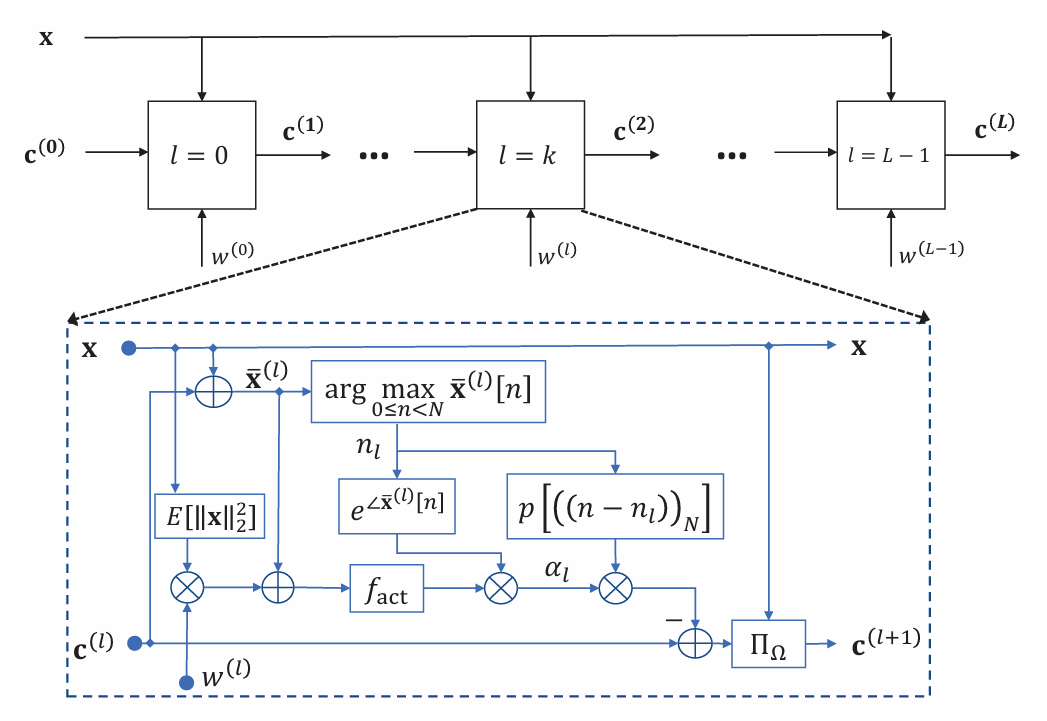
\includegraphics[width=0.75\linewidth]{Figures/37_pr_dun_architecture.png}
    \caption{Architecture of the PR-DUN (PAPR Reduction Deep Unfolding
             Network).  Each layer corresponds to one iteration of the
             projected gradient descent algorithm.  The step size $\mu^{(\ell)}$
             and potentially the threshold at each layer are trainable
             parameters optimized via backpropagation.
             Reproduced from~\cite{nguyen2022deep}.}
    \label{fig:prdun_architecture}
\end{figure}

PR-DUN unfolds $L$ iterations of the PGD algorithm into an $L$-layer
network.  The layer-$\ell$ computation is~\cite{nguyen2022deep}:
\begin{align}
    \bm{c}^{(\ell+\frac{1}{2})}
    &= \bm{c}^{(\ell)} - \mu^{(\ell)}
    \nabla_{\bm{c}}\bigl\|\bm{x} + \bm{c}^{(\ell)}\bigr\|_\infty^2,
    \label{eq:prdun_layer_grad} \\[6pt]
    \bm{c}^{(\ell+1)}
    &= \mathcal{P}_{\epsilon^{(\ell)}}\!\bigl(\bm{c}^{(\ell+\frac{1}{2})}\bigr),
    \label{eq:prdun_layer_proj}
\end{align}
where the \textbf{trainable parameters} at each layer are:
\begin{itemize}
    \item $\mu^{(\ell)}$: the gradient step size (controls how aggressively
          peaks are canceled).
    \item $\epsilon^{(\ell)}$: the power budget for the projection
          (may vary per layer for better convergence).
\end{itemize}

The transmitted signal after $L$ layers is:
\begin{equation}
    \bm{s} = \bm{x} + \bm{c}^{(L)}.
    \label{eq:prdun_output}
\end{equation}


% ----------------------------------------------------------------------------
\section{Training Procedure}
\label{sec:prdun_training}
% ----------------------------------------------------------------------------

The PR-DUN loss function directly minimizes the PAPR of the output
signal~\cite{nguyen2022deep}:
\begin{equation}
    \mathcal{L}_{\mathrm{PR\text{-}DUN}}
    = \mathrm{PAPR}\bigl(\bm{x} + \bm{c}^{(L)}\bigr)
    = \frac{\max_n|x(n) + c^{(L)}(n)|^2}
           {\frac{1}{N}\sum_{n=0}^{N-1}|x(n) + c^{(L)}(n)|^2}.
    \label{eq:prdun_loss}
\end{equation}

Training uses the Adam optimizer and randomly generated OFDM symbols.
Because each layer's computation is differentiable (including the projection),
gradients flow from the loss through all $L$ layers to update
$\{\mu^{(\ell)}, \epsilon^{(\ell)}\}_{\ell=1}^{L}$~\cite{nguyen2022deep}.

\begin{keyinsight}
    PR-DUN has dramatically fewer trainable parameters than PRNet or NN-SCF.
    With $L$ layers and 2 parameters per layer, there are only $2L$
    trainable parameters total (e.g., $2 \times 10 = 20$ for $L=10$).
    Compare this to PRNet's millions of weights.  This makes PR-DUN
    extremely fast to train and less prone to overfitting~\cite{nguyen2022deep}.
\end{keyinsight}


% ----------------------------------------------------------------------------
\section{Simulation and System Parameters}
\label{sec:prdun_params}
% ----------------------------------------------------------------------------

\begin{table}[H]
    \centering
    \caption{Simulation parameters for PR-DUN~\cite{nguyen2022deep}.}
    \label{tab:prdun_params}
    \begin{tabular}{@{} l l @{}}
        \toprule
        \textbf{Parameter} & \textbf{Value} \\
        \midrule
        Number of subcarriers ($N$) & 64, 128, 256 \\
        Modulation scheme & 16-QAM \\
        Oversampling factor & 4 \\
        Channel model & AWGN \\
        Number of unfolded layers ($L$) & 10 (evaluated) or 5--20 \\
        Trainable params per layer & 2 ($\mu^{(\ell)}$, $\epsilon^{(\ell)}$) \\
        Optimizer & Adam \\
        Learning rate & $10^{-3}$ \\
        Training set size & $10^5$ OFDM symbols \\
        Batch size & 256 \\
        Number of epochs & 100 \\
        Baselines compared & Clipping, SLM, TR, ICF \\
        \bottomrule
    \end{tabular}
\end{table}


% ----------------------------------------------------------------------------
\section{Results and Analysis}
\label{sec:prdun_results}
% ----------------------------------------------------------------------------

\subsection{PAPR Reduction Performance}

\begin{figure}[H]
    \centering
    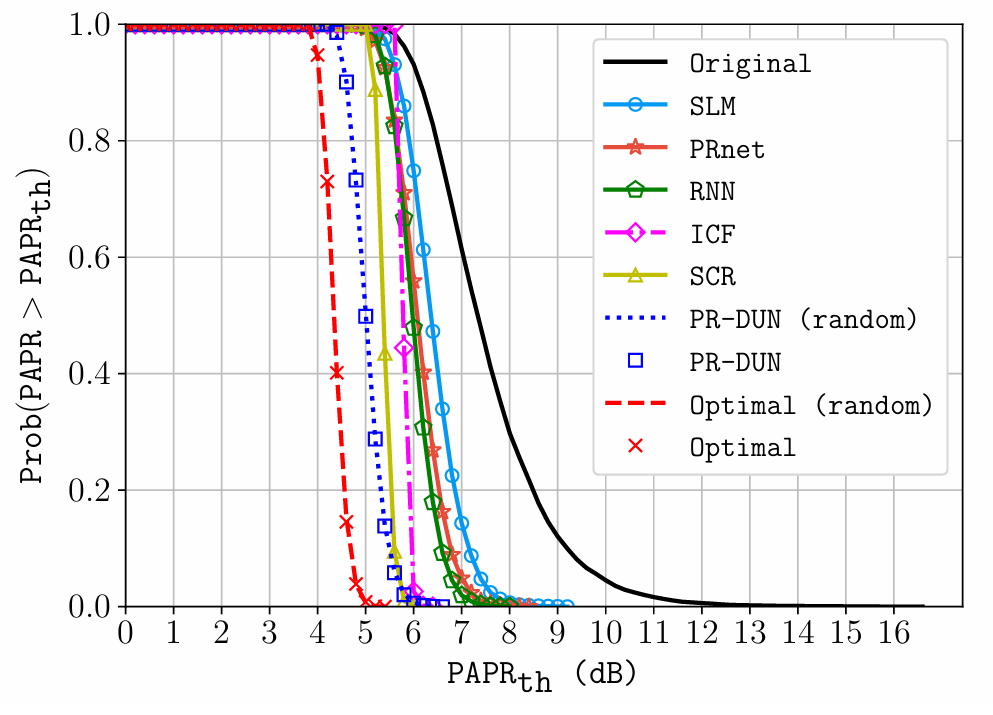
\includegraphics[width=0.70\linewidth]{Figures/41_pr_dun_ccdf.png}
    \caption{CCDF of PAPR for PR-DUN compared to conventional OFDM,
             clipping, SLM, and iterative clipping and filtering (ICF).
             PR-DUN achieves superior PAPR reduction with much lower
             complexity than ICF.
             Reproduced from~\cite{nguyen2022deep}.}
    \label{fig:prdun_ccdf}
\end{figure}

\subsection{Effect of Power Constraint}

\begin{figure}[H]
    \centering
    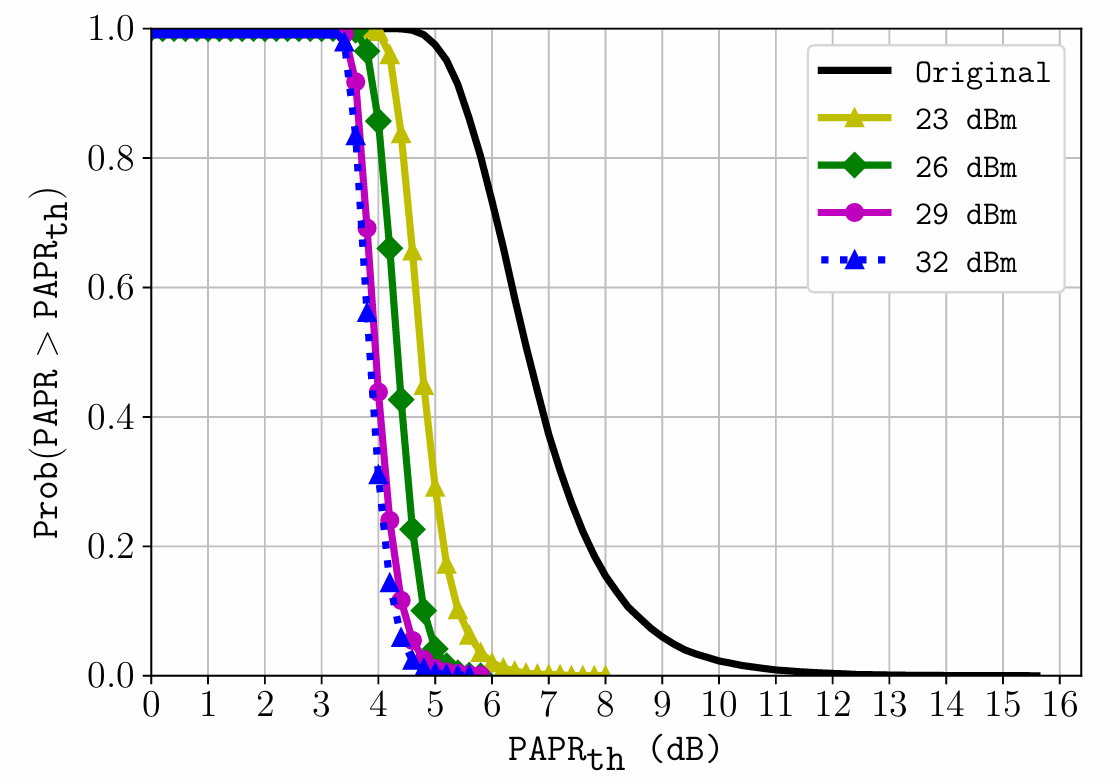
\includegraphics[width=0.70\linewidth]{Figures/38_pr_dun_papr_power.png}
    \caption{CCDF of PAPR for PR-DUN with different power constraint
             values.  A larger power budget $\epsilon$ allows more aggressive
             peak cancellation but increases signal distortion.
             Reproduced from~\cite{nguyen2022deep}.}
    \label{fig:prdun_ccdf_power}
\end{figure}

\subsection{BER Performance}

\begin{figure}[H]
    \centering
    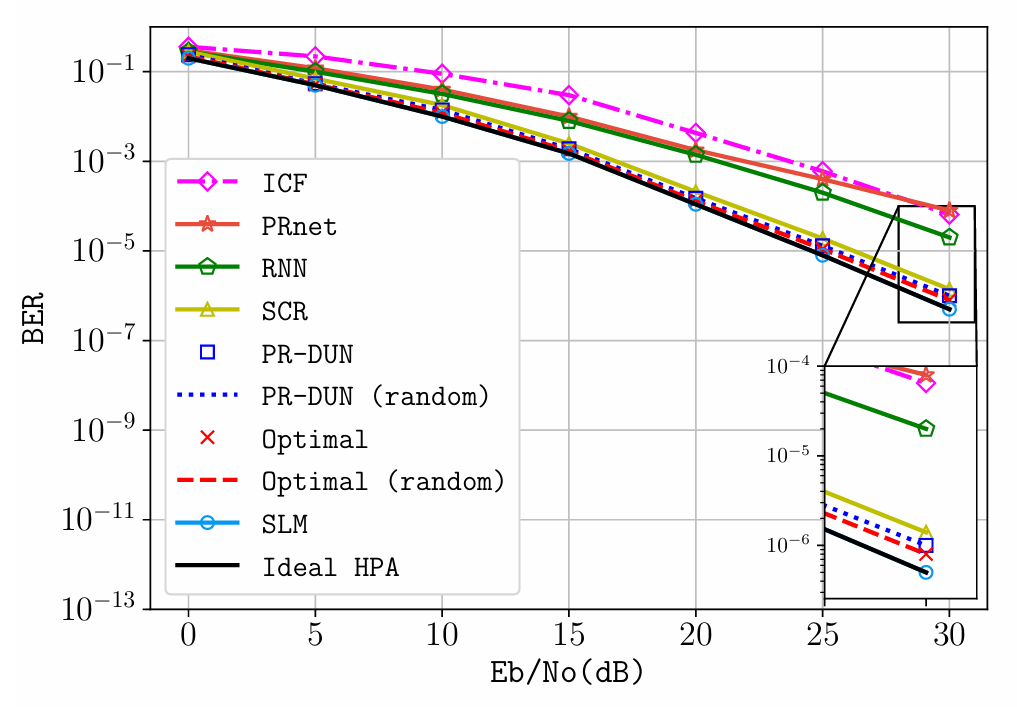
\includegraphics[width=0.70\linewidth]{Figures/42_pr_dun_ber.png}
    \caption{BER vs.\ SNR for PR-DUN.  The power constraint limits
             signal distortion, keeping the BER close to ideal OFDM.
             Reproduced from~\cite{nguyen2022deep}.}
    \label{fig:prdun_ber}
\end{figure}

\subsection{Complexity Comparison}

\subsection{Effect of Reserved Sub-carriers}

\begin{figure}[H]
    \centering
    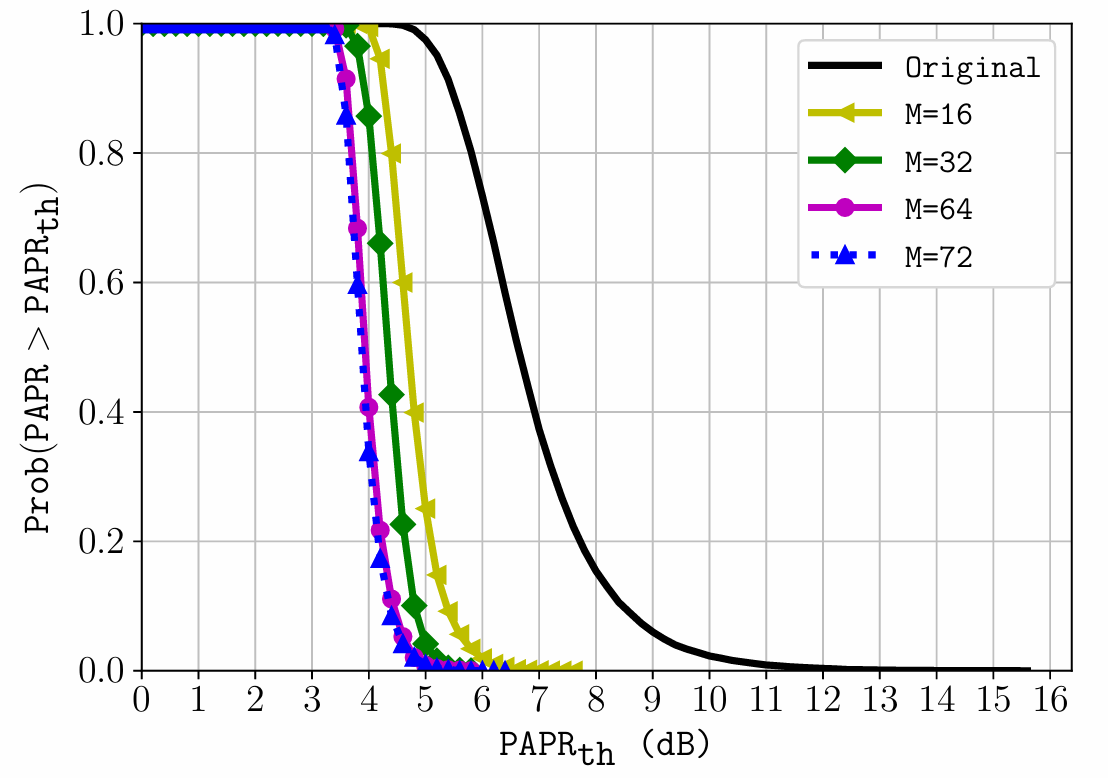
\includegraphics[width=0.70\linewidth]{Figures/40_pr_dun_papr_subcarriers.png}
    \caption{PAPR reduction for different numbers of reserved sub-carriers.
             More reserved sub-carriers leads to better PAPR reduction.
             Reproduced from~\cite{nguyen2022deep}.}
    \label{fig:prdun_subcarriers}
\end{figure}

\subsection{Effect of Number of Layers}

\begin{figure}[H]
    \centering
    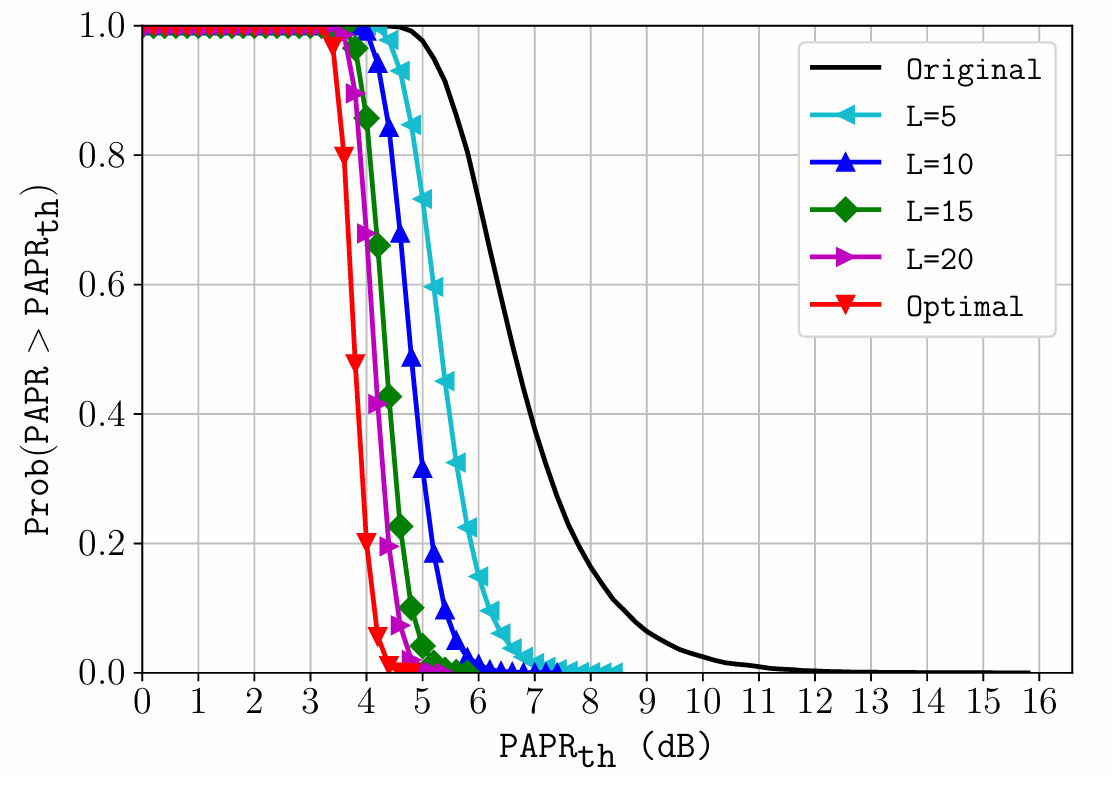
\includegraphics[width=0.70\linewidth]{Figures/39_pr_dun_papr_layers.png}
    \caption{PAPR reduction as a function of the number of unfolded layers
             $L$.  Performance improves rapidly up to $L \approx 10$, with
             diminishing returns beyond that.
             Reproduced from~\cite{nguyen2022deep}.}
    \label{fig:prdun_layers}
\end{figure}


% ----------------------------------------------------------------------------
\section{Common Misconceptions}
\label{sec:prdun_misconceptions}
% ----------------------------------------------------------------------------

\begin{misconception}
    \textbf{``PR-DUN is just a neural network with 20 parameters.''} \\
    While the number of \emph{trainable} parameters is small (e.g., 20),
    each layer performs significant computation: a full gradient evaluation
    (which involves comparing all $N$ signal samples) and a projection.
    The per-layer computational cost is comparable to one classical
    PGD iteration.  The ``intelligence'' lies not in network
    complexity but in the \emph{learned optimization} of per-layer
    parameters~\cite{nguyen2022deep}.
\end{misconception}


% ----------------------------------------------------------------------------
\section{Limitations and Open Problems}
\label{sec:prdun_limitations}
% ----------------------------------------------------------------------------

\begin{enumerate}
    \item \textbf{Signal distortion:}
          Unlike SLM, PR-DUN \emph{does} introduce distortion by adding
          a cancellation signal.  The power constraint $\epsilon$ controls
          the trade-off, but nonzero distortion is inherent~\cite{nguyen2022deep}.

    \item \textbf{AWGN-only evaluation:}
          Like PRNet, evaluations are limited to AWGN channels.

    \item \textbf{Fixed $L$:}
          The number of layers must be chosen beforehand.
          Adaptive termination (as in classical iterative algorithms)
          is not supported.

    \item \textbf{No side information handling:}
          PR-DUN generates a cancellation signal directly;
          it does not interact with the SLM framework.
\end{enumerate}


% ----------------------------------------------------------------------------
\section{Connection to Other Approaches}
\label{sec:prdun_connections}
% ----------------------------------------------------------------------------

PR-DUN stands out for its \textbf{model-driven} design:
\begin{itemize}
    \item Compared to PRNet and NN-SCF, it is more \textbf{interpretable}
          (each layer is a PGD iteration) and \textbf{parameter-efficient}
          ($2L$ vs.\ millions).
    \item Compared to GA-SLM, it is \textbf{faster at inference}
          (fixed $L$ layers vs.\ $P \times G$ evolutionary evaluations).
    \item Its main trade-off is that it introduces signal distortion
          (like clipping), whereas SLM-based approaches (GA-SLM, ESLM-AE)
          are distortion-free.
\end{itemize}

The final approach chapter (Chapter~\ref{ch:dl_ae_optical}) returns to
the autoencoder paradigm but in a new domain: coherent optical OFDM~\cite{alnaseri2025deep}.
